\documentclass[UTF8,a4paper,openany]{ctexbook}
\usepackage{pdfpages}
\usepackage{indentfirst}
\usepackage[hidelinks]{hyperref}
\usepackage{amssymb}
\usepackage{amsmath}
\usepackage{amsthm}
\DeclareMathOperator{\sign}{sign}

\usepackage{fontspec}
% switch to a monospace font supporting more Unicode characters
\setmonofont{FreeMono}
\usepackage{xcolor}
\usepackage{minted}
\newmintinline[lean]{lean4}{bgcolor=white}
\newminted[leancode]{lean4}{
	bgcolor=gray!10,
	fontsize=\normalsize,
	framesep=0pt,
}
\usemintedstyle{tango}  % a nice, colorful theme

% 页面边距
\usepackage[a4paper,left=2cm,right=2cm,top=2.5cm,bottom=2.5cm,headsep=0.98cm,footskip=1.75cm]{geometry}

% 行距
\usepackage{setspace}
\setstretch{1.25}

% 英文数字字体
\usepackage{fontspec}
\setmainfont{Times New Roman}

\newCJKfontfamily\qrthmchinese{SimHei}[AutoFakeBold=2]

% 标题格式
\usepackage{titlesec}

%%%%%%%%%%%%%%%%%%%%%%%%%%%%%%%%%%%%%%
%% 定理环境
%%%%%%%%%%%%%%%%%%%%%%%%%%%%%%%%%%%%%%

\newtheoremstyle{qrplain}
{0.5\baselineskip}
{0.5\baselineskip}
{\bfseries}
{}
{\qrthmchinese\bfseries}
{.}
{0.5em}
{}

\theoremstyle{qrplain}
\newtheorem{definition}{定义}[chapter]
\newtheorem{theorem}[definition]{定理}
{}
\renewenvironment{proof}[1][证明]
{\qrthmchinese\bfseries}
{\endgroup\hfill$\square$\par}

% 页眉页脚
\usepackage{fancyhdr}
\pagestyle{fancy}
\fancyhf{}
\fancyhead[C]{}
\fancyfoot[C]{\heiti\zihao{5}\thepage}
\renewcommand{\headrulewidth}{0.4pt}
\renewcommand{\footrulewidth}{0pt}
\fancypagestyle{plain}{%
	\fancyhf{}
	\fancyhead[C]{}
	\fancyfoot[C]{\heiti\zihao{5}\thepage}
	\renewcommand{\headrulewidth}{0.4pt}
	\renewcommand{\footrulewidth}{0pt}
}

%%%%%%%%%%%%%%%%%%%%%%%%%%%%%%%%%%%%%%
%% 一级标题（章）
%%%%%%%%%%%%%%%%%%%%%%%%%%%%%%%%%%%%%%

\titleformat{\chapter}
{\centering\heiti\zihao{3}} % 三号黑体居中
{第\chinese{chapter}章}
{0.5em}
{}

\titlespacing*{\chapter}
{0pt}{0.5em}{0.5em}

%%%%%%%%%%%%%%%%%%%%%%%%%%%%%%%%%%%%%%
%% 二级标题（节）
%%%%%%%%%%%%%%%%%%%%%%%%%%%%%%%%%%%%%%

\titleformat{\section}
{\songti\zihao{3}} % 三号宋体
{\thesection}
{0.5em}
{}

\titlespacing*{\section}
{0pt}{0.25em}{0.25em}

%%%%%%%%%%%%%%%%%%%%%%%%%%%%%%%%%%%%%%
%% 三级标题（小节）
%%%%%%%%%%%%%%%%%%%%%%%%%%%%%%%%%%%%%%

\titleformat{\subsection}
{\songti\zihao{4}} % 四号宋体
{\thesubsection}
{0.5em}
{}

% 缩进两个字符
\titlespacing*{\subsection}
{2em}{0.25em}{0.25em}

%%%%%%%%%%%%%%%%%%%%%%%%%%%%%%%%%%%%%%
%% 正文格式
%%%%%%%%%%%%%%%%%%%%%%%%%%%%%%%%%%%%%%

% 小四
\renewcommand\normalsize{\zihao{-4}}

% 首行缩进两个字符
\setlength{\parindent}{2em}
\setlength{\parskip}{0pt}

%%%%%%%%%%%%%%%%%%%%%%%%%%%%%%%%%%%%%%
%% 目录格式
%%%%%%%%%%%%%%%%%%%%%%%%%%%%%%%%%%%%%%

\usepackage{tocloft}

% 目录标题
\renewcommand{\contentsname}{目\quad 录}
\renewcommand{\cfttoctitlefont}{\hfill\heiti\zihao{-2}}
\renewcommand{\cftaftertoctitle}{\hfill}
\renewcommand{\cftdotsep}{1}

% 章目录格式
\renewcommand{\cftchapfont}{\heiti}
\renewcommand{\cftchappagefont}{\heiti}
\renewcommand{\cftchapleader}{\cftdotfill{\cftdotsep}}

% 节目录格式
\renewcommand{\cftsecfont}{\songti}
\renewcommand{\cftsecpagefont}{\songti}

% 小节目录格式
\renewcommand{\cftsubsecfont}{\songti}
\renewcommand{\cftsubsecpagefont}{\songti}

% 缩进
\cftsetindents{chapter}{0em}{0pt}
\cftsetindents{section}{1em}{0pt}
\cftsetindents{subsection}{2em}{0pt}

%%%%%%%%%%%%%%%%%%%%%%%%%%%%%%%%%%%%%%
%% 正文
%%%%%%%%%%%%%%%%%%%%%%%%%%%%%%%%%%%%%%

\begin{document}

\pagenumbering{gobble}
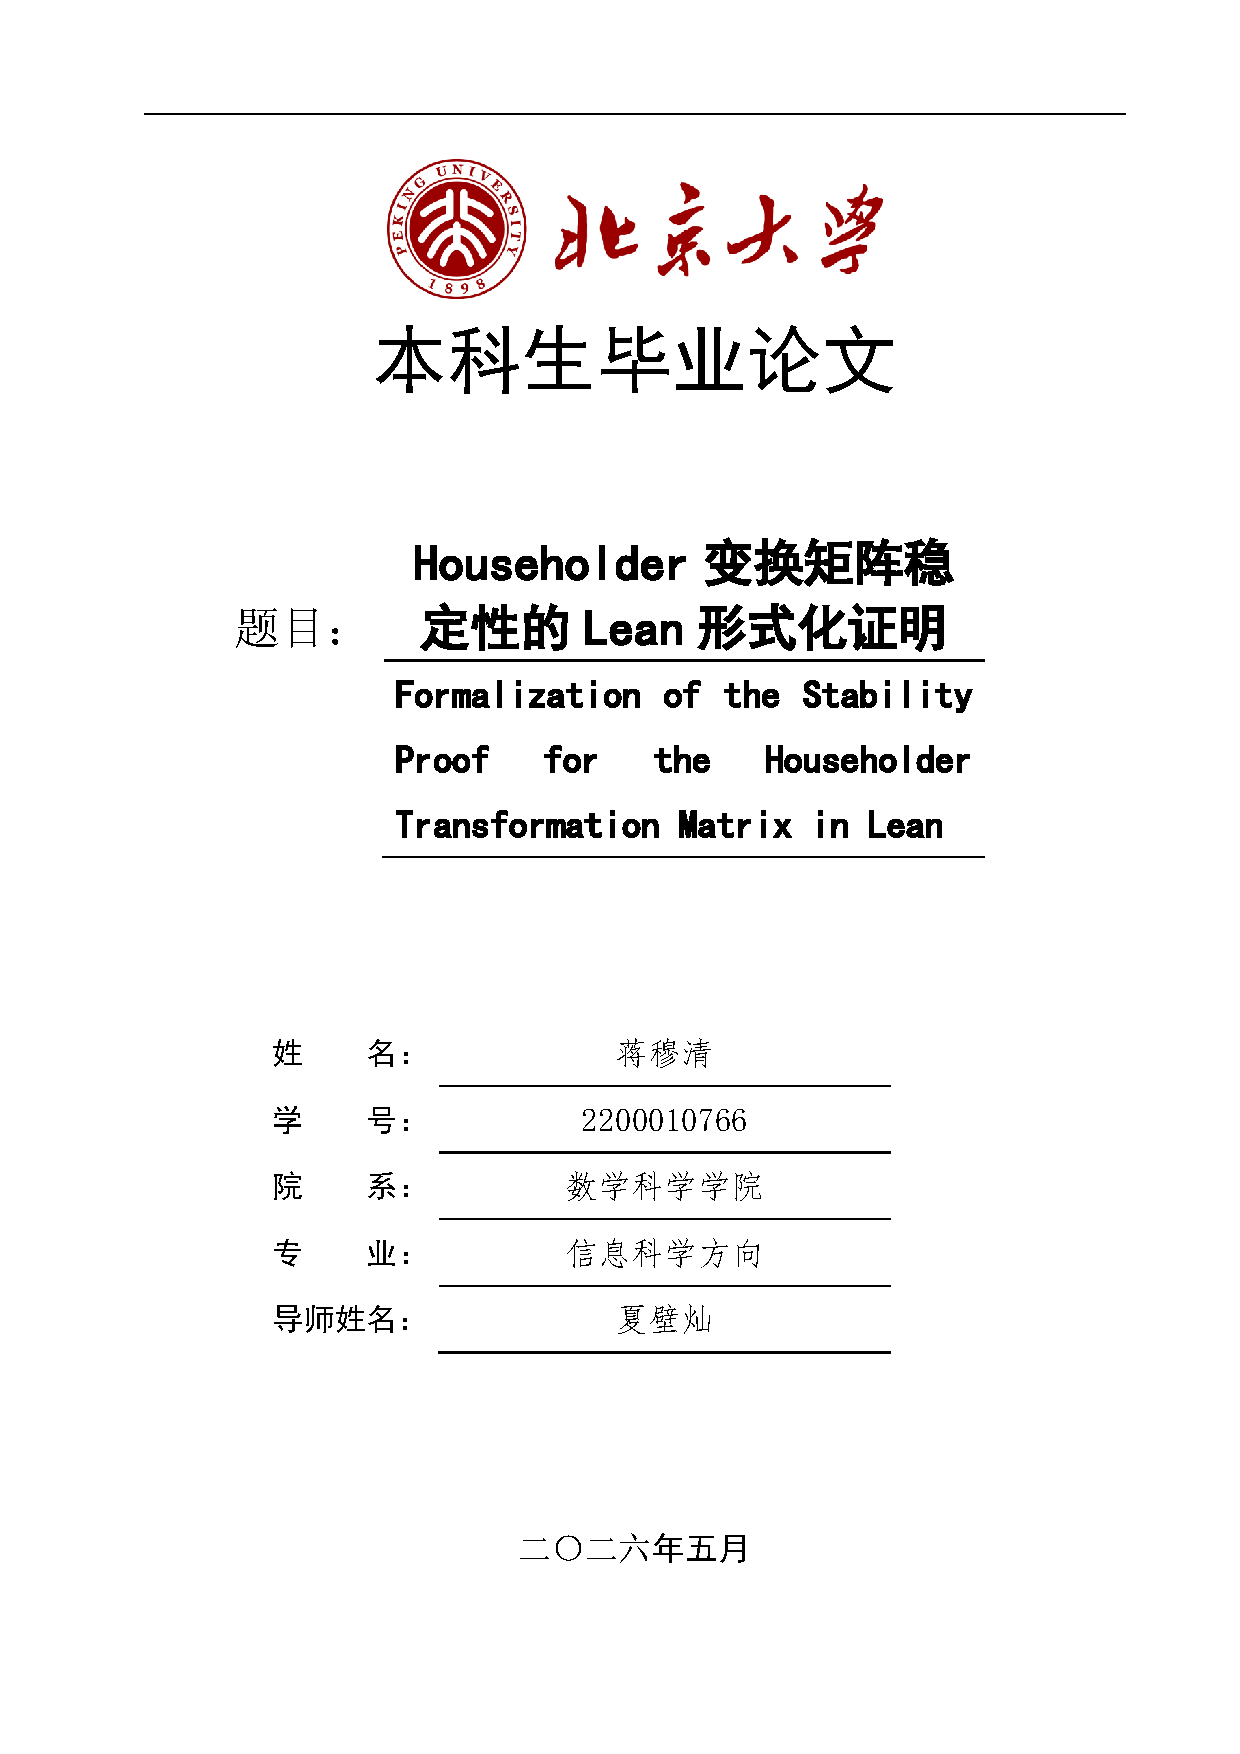
\includepdf[pages=-]{header.pdf}
\tableofcontents

\clearpage
\pagenumbering{arabic}

\chapter{引言}

\section{研究背景}

数值线性代数是科学计算的重要基础，在机器学习、计算机图形学、信号处理、工程仿真以及高性能计算等领域具有广泛应用。其中，QR分解作为数值线性代数中的核心工具，为线性方程组求解、最小二乘问题、特征值计算等任务提供了统一而高效的计算框架。

Householder变换是实现QR分解的重要方法。与经典Gram-Schmidt正交化相比，Householder方法能够有效减小浮点舍入误差带来的影响，因此在实际计算中被广泛采用。其核心思想是通过构造正交反射矩阵，将向量逐步变换为目标方向，从而实现矩阵的正交化过程。由于Householder方法涉及大量浮点运算，其数值稳定性分析一直是数值分析领域的重要研究内容。

传统数值分析通常通过数学推导对算法误差进行估计，并在一定假设条件下证明算法的稳定性。然而，这类证明往往包含复杂的符号推演与多层次误差传播分析，人工验证过程容易出现疏漏。因此，如何利用形式化方法对数值算法进行机器可验证的严格证明，逐渐成为形式化数学与可信计算研究中的重要方向。

近年来，定理证明辅助系统的发展为数学证明的形式化提供了有效工具。其中，Lean作为一种基于依赖类型理论的交互式定理证明系统，兼具较强的表达能力与较高的自动化水平，已被广泛应用于数学定理验证、程序正确性证明以及形式化数学库构建等领域。通过Lean对数值算法的稳定性结论进行形式化，不仅能够提高证明过程的可靠性，也有助于推动可信科学计算的发展。

\section{研究内容}

本文围绕 Householder 变换的数值稳定性问题展开研究，并基于Lean定理证明系统对相关结论进行形式化验证。研究的核心问题是：在浮点误差模型下，Householder 变换中关键向量的计算结果是否能够保持足够小的相对误差，以及如何以形式化方式严格证明该性质。

为此，本文首先对Householder变换的数学定义及其稳定性理论进行了分析，并建立相应的浮点误差模型。在此基础上，使用Lean对相关数学对象、误差界以及稳定性定理进行形式化表示与证明。本文进一步给出了误差界中的具体常数，从而使稳定性结论具有更明确的量化形式。这表明形式化方法不仅能够验证已有理论结果，还能够帮助将传统证明中被省略的步骤补全。

\chapter{理论基础}

本章与下一章中都将使用参考证明的源文献\textit{Accuracy and Stability of Numerical Algorithms}中的记号。

\section{Householder矩阵}

Householder矩阵是数值线性代数中一种重要的正交变换工具，广泛应用于QR分解等矩阵计算算法中。其核心作用是通过一种对称的“反射”变换，将向量或矩阵逐步转换为更便于计算的形式。相比Gram-Schmidt正交化等其他正交化方法，Householder法具有更好的数值稳定性，因此在现代科学计算软件与高性能数值计算中被广泛采用。

\subsection{定义与性质}

Householder矩阵（或称Householder变换矩阵）是具有如下形式的矩阵：
$$P=I-\frac{2}{v^Tv}vv^T,\quad 0\neq v \in \mathbb{R}^n$$
其对称性显然。又由
\begin{align*}
P^2&=I-\frac{4}{v^Tv}vv^T+\frac{4}{(v^Tv)^2}vv^Tvv^T\\&=I-\frac{4}{v^Tv}vv^T+\frac{4}{(v^Tv)^2}v(v^Tv)v^T=I
\end{align*}
结合其对称性可知其为正交矩阵。

\subsection{Householder变换}

考虑方程$Px=y$，其中$||x||_2=||y||_2$。我们令$P$为一个Householder矩阵。方程变为：$$x-2(\frac{v^Tx}{v^Tv})v=y$$

令$v=x-y$，我们有$$v^Tv=x^Tx+y^Ty-2x^Ty$$

又有$||x||_2=||y||_2$，即$x^Tx=y^Ty$。因此$$v^Tx=x^Tx-x^Ty=\frac{1}{2}v^Tv$$

从而$v=x-y$且$P=I-\frac{2}{v^Tv}vv^T$是方程的一个解。注意$x=y$时我们需要特别定义$P=I$防止出现除$0$的情况。

\section{QR分解}

QR分解是数值线性代数中的一种重要矩阵分解方法，在科学计算、数据分析、机器学习以及工程计算等领域具有广泛应用。通过QR分解，可以将一个复杂矩阵转化为更易处理的形式，从而便于求解线性方程组、最小二乘问题以及特征值问题等计算任务。QR分解在实际任务中非常重要，是现代数值算法中的基础工具之一。

\subsection{定义}

熟知对矩阵$A\in\mathbb{R}^{m\times n}$且$m\ge n$，总存在如下的分解：
$$A=QR=\left[\begin{matrix}Q_1&Q_2\\\end{matrix}\right]\left[\begin{matrix}R_1\\0\\\end{matrix}\right]=Q_1R_1$$

其中$Q\in\mathbb{R}^{m\times m}$为正交矩阵，$R_1\in\mathbb{R}^{n\times n}$为上三角矩阵。

\subsection{Householder矩阵在求解QR分解问题中的应用}
下面以一$4\times3$矩阵为例，展示Householder法求解QR分解问题的过程。
\begin{align*}
	A=&\left[\begin{matrix}\times&\times&\times\\\times&\times&\times\\\times&\times&\times\\\times&\times&\times\\\end{matrix}\right]\xrightarrow{P_1}\left[\begin{matrix}\times&\times&\times\\0&\times&\times\\0&\times&\times\\0&\times&\times\\\end{matrix}\right]\xrightarrow{P_2}\\
	&\left[\begin{matrix}\times&\times&\times\\0&\times&\times\\0&0&\times\\0&0&\times\\\end{matrix}\right]\xrightarrow{P_3}\left[\begin{matrix}\times&\times&\times\\0&\times&\times\\0&0&\times\\0&0&0\\\end{matrix}\right]=R
\end{align*}

一般地，我们考虑以下递归过程。记$A_1=A$。对递归的第$k$步，设我们面对如下矩阵：
$$A_k=\left[\begin{matrix}R_{k-1}&z_k&B_k\\0&x_k&C_k\\\end{matrix}\right],\quad R_{k-1}\in\mathbb{R}^{(k-1)\times(k-1)},x_k\in\mathbb{R}^{n-k+1}$$

其中$R_{k-1}$为上三角矩阵。那么令
$$P_k=\left[\begin{matrix}I_{k-1}&0\\0&\widetilde{P_k}\\\end{matrix}\right]$$

其中$\widetilde{P_k}$为求解$\widetilde{P_k}x_k=\sigma e_1$得到的Householder矩阵。这里$\sigma$可以取为任意值，只需保证$x_k\neq e_1$。

由2.1.2中提到的性质，我们知道不断重复次过程可以得到满足要求的QR分解。

注意在实际应用中，我们不会显式的将$P_k$计算出来，而是直接使用$\widetilde{P_k}C_k=C_k-\frac{2}{v^Tv}v(v^TC_k)$计算下一步递归。因此我们只需关注$v$的计算精度。

\section{浮点计算}

在现代计算机系统中，实数运算无疑在各类科学计算中都扮演重要的角色。然而，由于计算机硬件只能以有限位二进制形式存储数据，实数在机器中的表示不可避免地具有近似性。实践中计算机通常采用浮点数表示实数。浮点表示方法借鉴了科学计数法的思想，通过尾数与指数的组合实现对不同数量级实数的统一表示，从而成为现代计算机数值计算的核心基础。

尽管浮点表示极大提高了计算机处理实数的能力，但浮点计算误差问题始终是数值计算研究中的重要内容。由于浮点数只能对真实数值进行有限精度的近似表示，在数据存储、格式转换以及算术运算过程中都会产生误差。这些误差在大量迭代运算中可能不断累积与传播，从而影响最终计算结果的稳定性与可靠性。在高精度科学计算、数值模拟以及机器学习训练等场景中，微小的浮点误差甚至可能导致结果失真、算法不收敛或系统行为异常。因此，分析浮点误差的产生机制及其传播规律，对于提高数值计算的准确性与算法鲁棒性具有重要意义。

\subsection{浮点数存储}

计算机中的浮点数遵循 IEEE 754 标准，其存储结构主要由符号位、指数位和尾数位三部分构成。其中，符号位用于表示数值正负；指数位用于表示数值的数量级；尾数位用于存储有效数字。以单精度浮点数为例，其使用32个比特位存储一个实数。大部分浮点数（规格化浮点数）被表示为：
$(-1)^s\times(1.m)\times2^{e-127}$

其中$s, e, m$均为二进制串。它们长共为32位，构成了一个单精度浮点数。$s$表示符号位，占据1个比特位。$e$表示指数，占据8个比特位。$m$表示尾数，占据剩余的23个比特位。

\subsection{舍入误差}

分析如上的浮点数存储模型，我们很容易发现一些运算即使在运算数都是浮点数的情况下，得到的结果也无法用同样精度的浮点数存储。遇到这种情况时计算机会将其舍入到最接近的能被存储的实数并存储，这就造成了浮点数运算中的舍入误差。

我们考虑以下简化的模型中的一次计算。设我们有一个8位浮点数存储系统，8位由1位符号位，3位指数位和4位尾数位组成：
$$2^4\times1.1110+2^3\times1.0011=30+9.5=39.5=2^5\times1.001111$$

注意到这里最终的得数的尾数已经不能存入4位的尾数位了，因此强制被舍入：
$$2^5\times1.001111\approx2^5\times1.0100=40$$

这就是舍入误差的概念。虽然受限于浮点数存储系统，舍入误差无法避免，但它仍然具有一些性质，使我们可以对其进行分析，并控制误差。

\subsection{浮点计算误差模型}

注意到舍入误差只会发生在尾数位不够用的情况下，因此若我们使用m位尾数位的存储方法，每次舍入时产生的误差绝对值都不会超过原数字绝对值的$1/2^{m+1}$。由此我们可以采用以下的浮点误差描述模型：

设$x,\ y\in\mathbb{R}$，记$op\in\{+,-,\times,/\}$为基本浮点运算。本文采用如下经典浮点误差模型描述一次浮点运算的结果：
$$fl(x\ op\ y)=(x\ op\ y)(1+\delta),\quad |\delta|\le u$$

其中$u$是一个仅与浮点数存储系统有关的小正数。

注意到有一部分操作一定不会导致舍入误差，例如取相反数，或者与0相加等等。在后面的证明中会用到这一性质。

该模型的优势在于，它能够将一次浮点运算产生的误差统一表示为一个有界的相对扰动，从而使复杂算法中的误差传播分析可以转化为对多个扰动项的组合估计。相比直接分析底层二进制表示，该模型在保留主要误差特征的同时，大幅降低了理论分析的复杂度。此外，该模型中的误差界仅依赖于机器精度，而与具体运算数值无关，因此分析得到的结果对输入是鲁棒的。在后续证明中，本文将反复利用该模型对连续浮点运算中的误差进行估计，并给出误差的上界。

\chapter{Householder法的误差估计}

本章陈述本项目核心内容，证明使用Householder法得到的确定Householder矩阵的向量$v$的误差关于$n$和$u$的明确上界。

\section{记号}

\begin{definition}
	浮点计算精度u
\end{definition}
\begin{leancode}
variable (u : NNReal)
\end{leancode}
浮点误差模型部分和上一章中定义相同，不再赘述。

\begin{definition}
	记$\gamma_n=nu/(1-nu)$
\end{definition}
\begin{leancode}
def γ (n : ℕ) : ℝ := (n : ℝ) * (u : ℝ) / (1 - (n : ℝ) * (u : ℝ))
\end{leancode}
为n次浮点舍入后计算结果与正确结果的相对误差。书中为避免对常数的讨论，还定义了$\widetilde{\gamma_n}=\gamma_{cn}$。本文由于在所有需要使用这个参数的地方都已经将常数$c$显式计算出来，因此不再使用此参数。

对于某个特定的运算序列，我们用
$$|\theta_n|\le\gamma_n,\quad\theta_n\in\mathbb{R}$$
表示该运算序列中可能引入的误差。下文所有$\theta$默认满足此条件。

\begin{definition}
	符号函数
\end{definition}
我们规定
$$
\sign(x)=
\begin{cases}
1, & x \ge 0 \\
-1, & x < 0
\end{cases}
$$

注意这个sign的定义与通常的sign在$0$处定义不同。这个函数旨在防止在$x_1=1$时发生退化导致除$0$。

对于计算过程中的任意中间值$a$，我们记$a$为其在精确计算时得到的结果，$\hat{a}$为其在有浮点误差的环境中计算得到的结果。

\section{Householder过程}

对$x\in\mathbb{R}^n,\quad x\neq0$，我们使用如下的Householder算法来取得满足$\left(I-vv^T\right)x=-\left(\sign x_1\right)||x||_2e_1$的v：
$$
\left\{
\begin{array}{l}
v = x \\
l' = v^T v \\
l = \sqrt{l'} \\
s = \operatorname{sign}(x)\cdot l \\
v_1 = x_1 + s \\
p = s v_1 \\
\beta = 1/p \\
b = \sqrt{\beta}
\end{array}
\right.
$$

% 把这段写成更正式的证明
注意到进行到$v_1=x_1+s$一步结束时，$v=x-(-\left(\sign x_1\right)||x||_2e_1)$。由2.1.2节可知，此时有$P=I-\frac{2}{v^Tv}vv^T$是一个解。

又注意到这时$p=sv_1=sx_1+s^2$，$v^Tv=x^Tx+2s x_1+s^2=2sx_1+2s^2=2p$。从而$b=\sqrt\frac{2}{v^Tv}$在最后一步相当于一个归一化因子，使得Householder矩阵$P=I-\frac{2}{v^Tv}vv^T$变为计算中更简便的$P=I-vv^T$的简单形式。

\chapter*{参考文献}
\addcontentsline{toc}{chapter}{参考文献}

[1] Nicholas G. Higham (2002). \textit{Accuracy and Stability of Numerical Algorithms (Second Edition)}, 61-76, 353-362. Society for Industrial and Applied Mathematics.

[2] Guoxiong Gao, Haocheng Ju, Jiedong Jiang, Zihan Qin, Bin Dong (2024). A Semantic Search Engine for Mathlib4. \textit{EMNLP 2024 findings}. \url{https://arxiv.org/abs/2403.13310}.

[3] Lean and Mathlib4 Maintainer team. Documentation page for Mathlib4 and Lean, \url{https://leanprover-community.github.io/mathlib4_docs}


\chapter*{附录}
\addcontentsline{toc}{chapter}{附录}

\chapter*{致谢}
\addcontentsline{toc}{chapter}{致谢}


\includepdf[pages=-]{footer.pdf}

\end{document}